% id: 48-17
% book: 쎈B 대수 · 04 로그함수
% section: 유형 04 로그함수의 그래프 위의 점
% figure: tikz:fig-48-17
% answer: 
% answer_source: 
% variant_level: 0 (원본 전사)
% 이 파일은 build.mjs 가 items.json 에서 만든다. 고칠 때는 items.json 을 고친다.
\noindent\begin{minipage}[t]{0.58\linewidth}\vspace{0pt}\raggedright 오른쪽 그림과 같이 함수 $y=\log_3 x$의 그래프 위의 점~$\pt{A}$와 $x$축 위의 두 점~$\pt{B}$, $\pt{C}$에 대하여 사각형~$\pt{ABCD}$가 한 변의 길이가 $2$인 정사각형일 때, $\pt{D}(p{,}\mkern3mu\mathopen{}q)$이다. 이때 $p+q$의 값은?\end{minipage}\hfill\begin{minipage}[t]{0.4\linewidth}\vspace{0pt}\centering \resizebox{\ifdim\width>\linewidth\linewidth\else\width\fi}{!}{% 48-17(48쪽) — $y=\log_3 x$ 의 그래프 위의 점 A 와 $x$축 위의 두 점 B, C 로 만든 정사각형 ABCD(원문 「오른쪽 그림」). 스캔 화질이 낮아 TikZ 로 다시 그림.
% 라벨은 원문에 있는 것만 — 곡선 이름 $y=\log_3 x$, 꼭짓점 A·B·C·D, 원점 O. $p$, $q$(답)는 그림에서 읽히지 않게 적지 않는다.
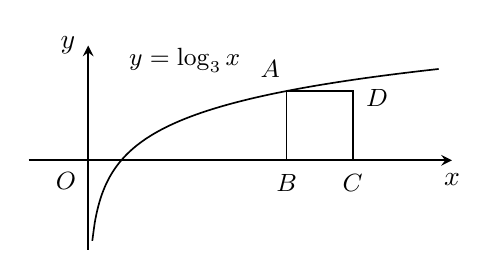
\begin{tikzpicture}[line width=0.6pt, x=0.42cm, y=0.54cm, >=stealth]
  \draw[->, line width=0.7pt] (-1.8,0) -- (11.0,0) node[below=1pt] {$x$};
  \draw[->, line width=0.7pt] (0,-2.1) -- (0,2.7) node[left=1pt] {$y$};
  \draw[domain=0.125:10.6, samples=140, smooth] plot (\x, {ln(\x)/ln(3)});
  \draw (6.0,0) -- (6.0,1.6309) -- (8.0,1.6309) -- (8.0,0) -- cycle;
  \node[font=\small, anchor=south east] at (6.10,1.72) {$\pt{A}$};
  \node[font=\small, anchor=west] at (8.10,1.46) {$\pt{D}$};
  \node[font=\small, anchor=north] at (6.0,-0.10) {$\pt{B}$};
  \node[font=\small, anchor=north] at (8.0,-0.10) {$\pt{C}$};
  \node[font=\small, anchor=north east] at (-0.06,-0.06) {$\pt{O}$};
  \node[font=\small, anchor=south east] at (4.90,1.84) {$y=\log_3 x$};
\end{tikzpicture}
}\end{minipage}\par
\dmchoicesauto{}{$10$}{$11$}{$12$}{$13$}{$14$}
